% Lorentz.tex      pdflatex ZhCvGo15
% Diffuse globally, compute locally: a cyclist tale
% Tingnan Zhang, Daniel I. Goldman and Predrag Cvitanovi\'c

%\section{Diffusion in periodic arrays}
%\label{s-Lorentz}

\begin{figure}[htbp]
  \begin{center}
    (a)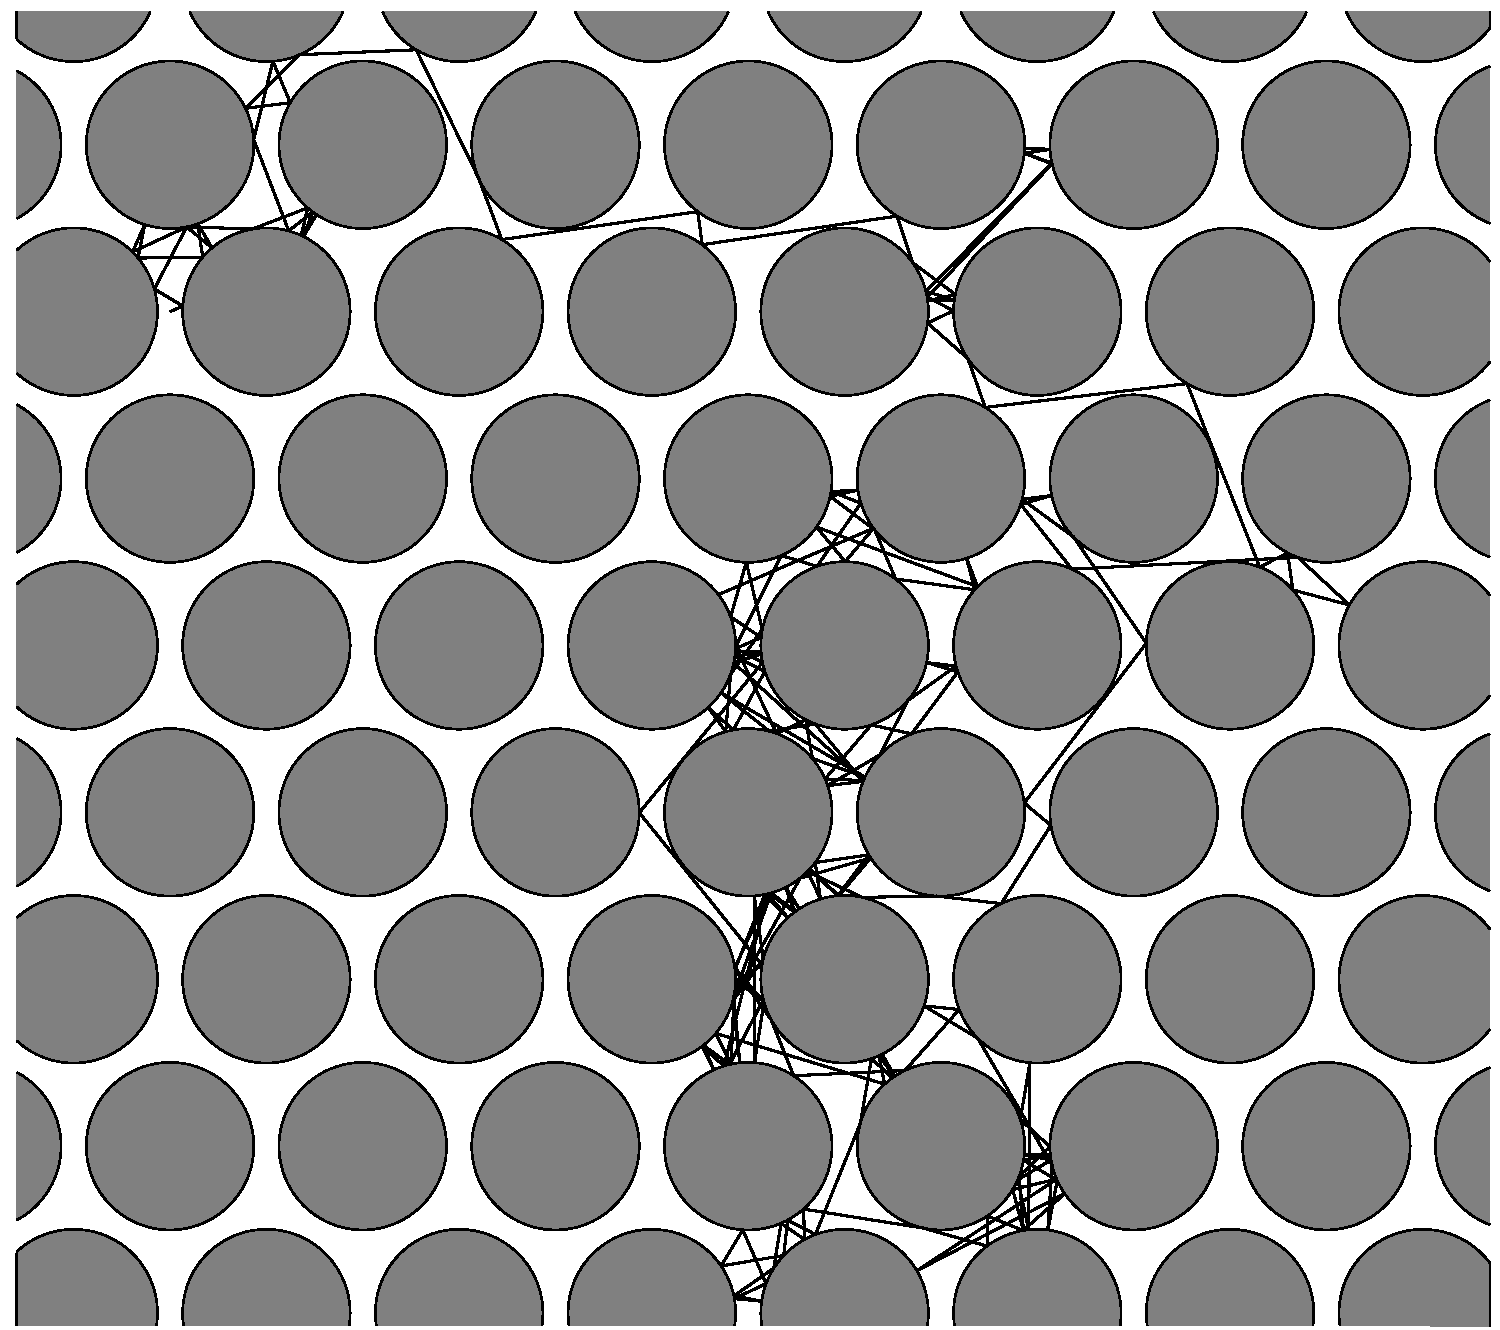
\includegraphics[width=0.45\textwidth]{diffuseChaoticBouncing}
    (b)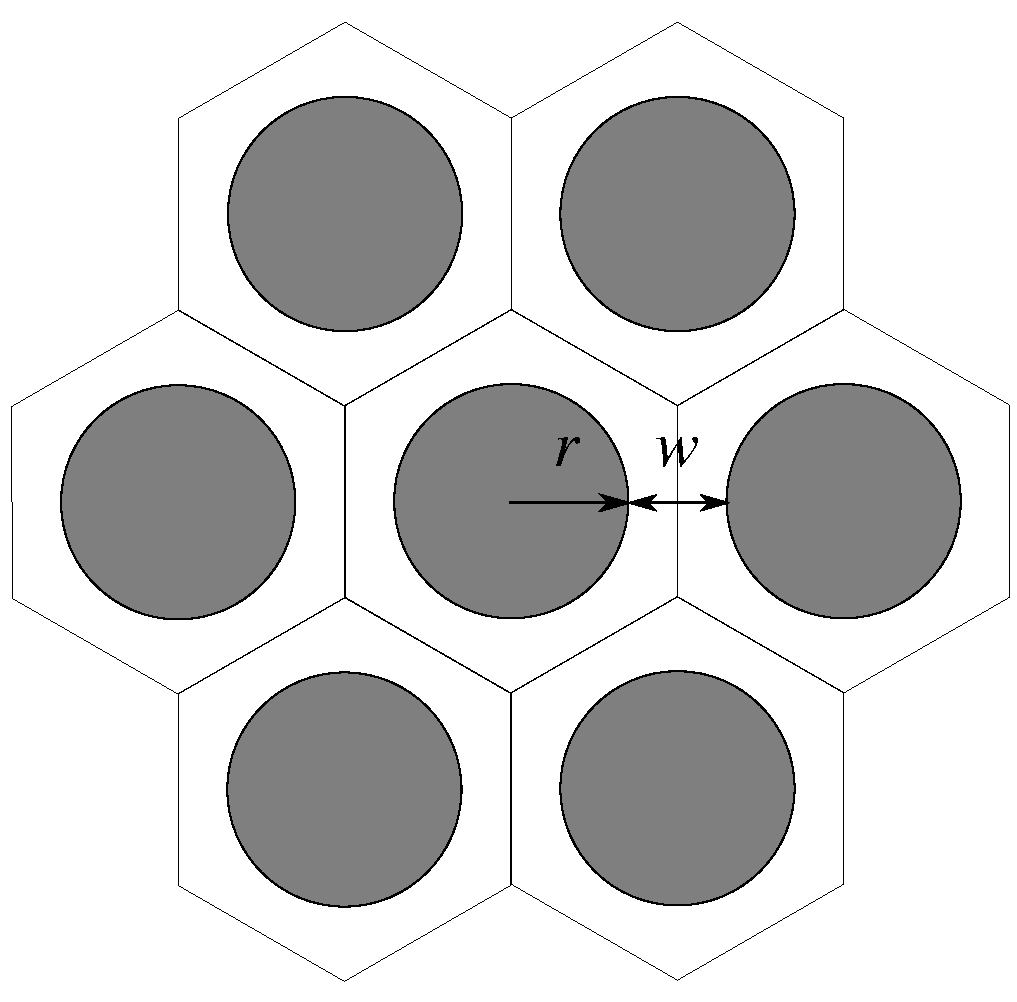
\includegraphics[width=0.45\textwidth]{diffuseLorentzGasParams}
  \end{center}
  \caption[]{\label{fig-chaoticBouncing}
  Motion in the Lorentz gas system. (a)  The chaotic trajectory of a
  ``gas'' particle bouncing in the array of disks  arranged in a
  hexagonal lattice pattern. The distance between disks are close  enough
  such that the particle has no infinite free flight (finite horizon).
  (b) A portion of the triangular Lorentz gas    system. The ratio of
  distance $w$ between the nearest pair of disks to the    disk radius
  $r$ determines the dynamical properties in the system.
  }
\end{figure}
    \PC{2015-10-21} {make our own \reffig{fig-chaoticBouncing}\,(a), otherwise
    we have to ask J.-P. Eckmann for permission to use it. It has not been
    published. Similarly, we need our own \reffig{fig-chaoticBouncing}\,(b),
    I do not remebr where this one is from.}

One distinguishes
the {\em infinite horizon} diffusive behavior, which allows for infinite
length flights, from
the {\em finite horizon} case, where the particle always
hits the next disk in finite time.
Here we shall restrict
our consideration to the finite horizon case,
with disks sufficiently
large so that no infinite length free flight is possible.
In this case the diffusion is normal, with $\hat{x}(t)^2$
growing like $t$.


\bigskip
=========== TO REUSE ========

    \PC{2015-10-21}
    {edits based Cvitanovi\'c,  Eckmann,and Gaspard\rf{LorentzDiff}}
The lattice symmetry of the Lorentz billiard has important consequence on
the properties of the function $Q(\beta)$ are best illustrated by
introducing its analytic continuation at $\beta = i k$.  The function
$F(k)=Q(ik)$ is the rate associated with the incoherent scattering
function $\langle \exp i k \cdot (\hat x_t - x) \rangle_M$ considered in
light or neutron scattering experiments in liquids, in particular, by Van
Hove\rf{BoonYip80,VanHove54}. The vector $k$ is interpreted as the
wavenumber of the hydrodynamic modes of diffusion which we also find in
the Lorentz gas.  The function $F(k)$ turns out to be a dispersion
relation since $F(k)=-D k^2 + {\cal O}(k^4)$ in an isotropic diffusive
system.  The isotropy of a liquid implies that the dispersion relation
only depends on the amplitude $\vert k\vert$ of the wavenumber.


On the other hand, the lattice symmetry of the Lorentz gas
imposes special restrictions on the properties of the dispersion relation
$F(k)$ and on the values taken by the wavenumber.  The present classical
problem of diffusion is similar to the quantum motion of a particle in a
periodic potential.  Hence, the wavenumber takes its values in the so-called
Brillouin zone\rf{BoSmWi36,Harrison70}.  A mode of diffusion is associated with each value of
the wavenumber $k$ so that the direction of $k$ is privileged in the
system.  As a consequence, the symmetry of the lattice is reduced by the choice
of $k$.  This symmetry reduction is formalized by the concept of little group
associated with the wavenumber $k$, which is the subgroup of the lattice point
group leaving invariant the vector $k$.  For most values of $k$ inside the
Brillouin zone, the little group is trivial because it contains only the
identity.  However, the little group is larger when the wavenumber belongs to
special symmetry lines or symmetry points in the Brillouin zone.  In particular,
the little group coincides with the full point group when $k=0$.

The preceding considerations concern the consequences of the lattice symmetry
on the factorization of the zeta function.  There is a different problem which
is to express the zeta function in terms of the prime periodic orbits of the
fundamental domain $\tilde M$ of the lattice (see Fig. 2) rather than
those of the elementary (Wigner-Seitz) cell $M$.
%This problem is a priori independent of the factorization
%discussed above and presents the following difficulty.
Here the stumbling block appears to be
the breaking of the rotational symmetry by
the auxilliary vector $\beta$, or, in other words,
the non-commutativity of translations and rotations.
More precisely, the global distance
$ \hat\phi^{r \period{\tilde{p}}} (\tx{\tpk}) - \tx{\tpk} $, $\tx{\tpk} \in \tp$,
% $ \hn_{r |\t p|}(\tx{\tpk}) $
depends on the starting cycle point if
$\tp$ is only a segment of the global cycle $p$. An
example is the diamond-shaped cycle of Fig.~3;
%the problem is that the $\tp$ segment of
%the global trajectory is not a translation in $\hM$.
depending whether one starts at $\tx_1$ or $\tx_2$, the global
distance covered in time $\period{\tilde{p}}$ is either the short or the
long diagonal.

In triangular and square lattices the diffusion is isotropic, but the
full function $Q(\beta)$ contains more information on the lattice
symmetry than the diffusion matrix of the second derivatives of
$Q(\beta)$. The behavior of the function $Q(\beta_x, \beta_y)$ away from
$\beta=0$ is discussed in \refref{Gaspard92a}. \PC{2015-12-03}{Lattice
gases literature (Hasslacher, Frisch?) has a reference to a formula in
Landau-Lifshitz that shows triangular lattice is isotropic - try to
re-find this.}

Compared to earlier literature\rf{CvitaEckardt,robb}, the new feature of the
problem at hand is use of vector-valued functions. The arbitrary vector
$\beta$ is only a device for generating moments~--~the moments themselves
are invariant under discrete symmetries, but it can be interpreted in
terms of the wavenumber of the hydrodynamic modes of diffusion.

The stumbling block
appears to be
 the breaking of the rotational symmetry by
 the auxilliary vector $\beta$, or, in other words,
the non-commutativity of translations and rotations.
More precisely,
in contrast to Eq.~(11), the global distance
$ \hf^{r \period{\tilde{p}}} (\tx{\tpk}) - \tx{\tpk} $, $\tx{\tpk} \in \tp$,
 $ \hn_{r |\t p|}(\tx{\tpk}) $
depends on the starting cycle point if
$\tp$ is only a segment of the global cycle $p$. An
example is the diamond-shaped cycle of Fig.~3;
the problem is that the $\tp$ segment of
the global trajectory is not a translation in $\hM$.
depending whether one starts at $\tx_1$ or $\tx_2$, the global
distance covered in time $\period{\tilde{p}}$ is either the short or the
long diagonal. We have not found a natural way of associating
a global distance in  formula Eq.~(17) with a fundamental domain
cycle $\tp$.

    \PC{2015-10-21}
    {the text from Cvitanovi\'c, Gaspard and Schreiber\rf{CGS92}}
In the periodic Lorentz gas\rf{Lorentz1905}
a point particle reflects elastically off
a periodic array of reflecting disks in a plane.
The system can
be thought of as an unfolding of the Sinai billiard\rf{Sinai70}.
The standard diffusion constant can be defined if the particle has a bounded
free path between any two successive bounces.
An example is a triangular array with sufficiently small
inter-disk spacing.
Unfortunately, as we shall see,
the same mechanism that guarantees a finite horizon
also leads to rather awkward pruning of periodic orbits.
